\documentclass[a4paper,12pt]{report}
\usepackage[margin=2cm]{geometry}
\usepackage[utf8]{inputenc}
\usepackage{listings}
\usepackage{color}
\usepackage{xcolor}
\usepackage{hyperref}
%\usepackage{zeta}
%\usepackage[inline]{trackchanges}
\usepackage{pgf,pgfarrows,pgfnodes,pgfautomata,pgfheaps}
%\usepackage{makeidx}
%\usepackage{tocloft}
%\usepackage{romanian}
\usepackage{pdfpages}
\usepackage{graphicx}
\usepackage{mathtools}
\usepackage{url}
\graphicspath{ {fig/} }

\definecolor{codegreen}{rgb}{0,0.6,0}
\definecolor{codegray}{rgb}{0.5,0.5,0.5}
\definecolor{codepurple}{rgb}{0.58,0,0.82}
\definecolor{backcolour}{rgb}{0.95,0.95,0.92}

\lstdefinestyle{mystyle}{
backgroundcolor=\color{backcolour},
commentstyle=\color{codegreen},
keywordstyle=\color{magenta},
numberstyle=\tiny\color{codegray},
stringstyle=\color{codepurple},
basicstyle=\footnotesize,
breakatwhitespace=false,
breaklines=true,
captionpos=b,
keepspaces=true,
numbers=left,
numbersep=5pt,
showspaces=false,
showstringspaces=false,
showtabs=false,
tabsize=2
}

\lstset{style=mystyle}

\usepackage[backend=bibtex, style=alphabetic, sorting=ynt]{biblatex}
\addbibresource{BOC_2013.bib}
\begin{document}
\newcommand{\h}{\texttt}

\vspace{-5cm}
\begin{center}
Department of Computer Science\\
Technical University of Cluj-Napoca%\\https://www.overleaf.com/project/5c7f87ea86f3ee70d98c7434
\pgfimage[width=10cm]{fig/footer}
\end{center}
\vspace{1cm}
%\maketitle
\begin{center}
\begin{Large}
Knowledge-Based Systems\\
\end{Large}
Laboratory activity\\


Ontology title: \textbf{TES V: Skyrim Skill Tree}\\
Team name: \textbf{Dovahyol}\\
Students: Coman Nicolae\\
Zavaczki Peter\\
Email: ncoman32@yahoo.com\\
peter.zavaczki@gmail.com\\

\vspace*{14cm}

Assoc. Prof.dr. eng. Adrian Groza\\
Adrian.Groza@cs.utcluj.ro
\end{center}

\newpage

\tableofcontents
\clearpage
\chapter{Contents}
\section{Competency questions}
Use cases:

\begin{itemize}
\item Anyone who wants to play the game TES V: Skyrim.
\item Anyone who wants to know which skills can be learnt at current level.
\item Anyone who wants to know what perks the skills provide.
\item Anyone who wants to know suitable skills based on the character's build.
\item Anyone who wants to know the pre-required skill in order to learn a specific skill.
\item Anyone who wants to know the level required to learn a specific skill.
\item Anyone who wants to know the skills not worth prioritizing.
\end{itemize}

\hfill \break
Competency questions:

\begin{itemize}
\item What are the classes of characters I can play?
\item What are the skills suitable for build X?
\item Should I invest in skill tree X if my character is build Y?
\item What skills can I unlock at level X?
\item What skill is required for unlocking skill X?
\item What level is required for unlocking skill X?
\item What are the perks provided by skill X?
\end{itemize}


\clearpage
\section{Related ontologies}
The ontologies we found were related to ours based on the fact that they all tackle the topic of video games.

\begin{itemize}
\item Dota 2 ontology - An ontology describing a scenario from the game - \url{https://ontohub.org/repositories/dota-2-ontology}
\item Core Game Ontology - An ontology classifying games by their properties - \url{http://autosemanticgame.institutedigitalgames.com/ontologies/core-game-ontology/}
\item Dota 2 item ontology - An ontology about the items and builds in Dota 2 - \url{https://ontohub.org/boc2018/Dota\%202\%20Item\%20ontology}
\end{itemize}

Unfortunately none of these ontologies are useful to us, as we tackle a very specific topic. None of them will be used.


\clearpage
\section{Tbox}
Our main concepts are Skill\_class, Skill, Build and Race. The figure below shows the concepts in a more detailed way.

\begin{figure}[h]
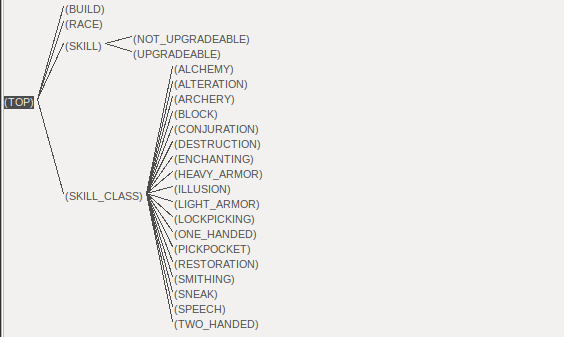
\includegraphics[scale=0.65]{taxonomy}
\end{figure}

The Skill\_class is split into the existing 12 disjoint classes: Archery, Block, Heavy Armor, One-handed, Smithing, Two-handed, Alteration, Conjuration, Destruction, Enchanting, Illusion, Restoration, Alchemy, Light Armor, Lockpicking, Pickpocket, Sneak and Speech. These skill classes contain skills. Builds are paired with skill classes to tell what skill class is suitable for what build.

\begin{lstlisting}
(IMPLIES SNEAK SKILL_CLASS)
(IMPLIES LOCKPICKING SKILL_CLASS)
(IMPLIES PICKPOCKET SKILL_CLASS)
(IMPLIES SPEECH SKILL_CLASS)
(IMPLIES ALCHEMY SKILL_CLASS)
(IMPLIES ILLUSION SKILL_CLASS)
(IMPLIES CONJURATION SKILL_CLASS)
(IMPLIES DESTRUCTION SKILL_CLASS)
(IMPLIES RESTORATION SKILL_CLASS)
(IMPLIES ALTERATION SKILL_CLASS)
(IMPLIES ENCHANTING SKILL_CLASS)
(IMPLIES SMITHING SKILL_CLASS)
(IMPLIES HEAVY_ARMOR SKILL_CLASS)
(IMPLIES BLOCK SKILL_CLASS)
(IMPLIES TWO_HANDED SKILL_CLASS)
(IMPLIES ONE_HANDED SKILL_CLASS)
(IMPLIES ARCHERY SKILL_CLASS)
(IMPLIES LIGHT_ARMOR SKILL_CLASS)
(DISJOINT SNEAK LOCKPICKING PICKPOCKET SPEECH ALCHEMY ILLUSION CONJURATION DESTRUCTION RESTORATION ALTERATION ENCHANTING SMITHING HEAVY_ARMOR BLOCK TWO_HANDED ONE_HANDED ARCHERY LIGHT_ARMOR)

(define-primitive-role isSuitable :domain SKILL_CLASS :range BUILD)
\end{lstlisting}

Skills can be either Upgradeable or Not\_upgradeable, these two traits are obviously disjoint between eachother. Above this, we need to model the pre-required skill, for which we use a role called \textit{hasSkillRequirement}. For the level requirement and perk description we use attributes.

\begin{lstlisting}
(IMPLIES UPGRADEABLE SKILL)
(IMPLIES NOT_UPGRADEABLE SKILL)
(DISJOINT NOT_UPGRADEABLE UPGRADEABLE)

(define-primitive-role hasSkillRequirement :domain SKILL :range SKILL)

(define-concrete-domain-attribute hasLevelRequirement :TYPE INTEGER)
(define-concrete-domain-attribute hasDescription :TYPE STRING)
\end{lstlisting}

%\clearpage
\section{Abox}
Our Abox is mainly composed of instances of skills, then some races and some builds.
Instances of races and builds are simple, since they are then used to determine which skill class to invest in.
An instance of a race and one of a build:

\begin{lstlisting}
(INSTANCE REDGUARD RACE)

(INSTANCE BARBARIAN BUILD)
\end{lstlisting}

An instance of a skill:

\begin{lstlisting}
(INSTANCE ADEPT_ALTERATION SKILL)
(INSTANCE ADEPT_ALTERATION ALTERATION)
(RELATED ADEPT_ALTERATION APPRENTICE_ALTERATION hasSkillRequirement)
(ATTRIBUTE-FILLER ADEPT_ALTERATION 50 hasLevelRequirement)
(ATTRIBUTE-FILLER ADEPT_ALTERATION "Cast Adept level Alteration spells for half magicka." hasDescription)
\end{lstlisting}

This can be seen in the tree structure in the images below. The skill is only the root, but since the skill requirement takes another skill as parameter, it extends until it reaches a "leaf skill".

\begin{figure}[h]
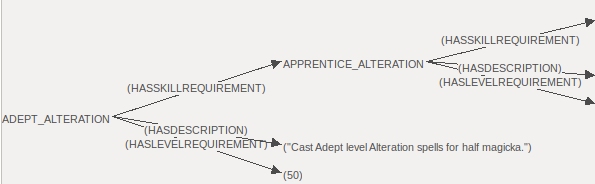
\includegraphics[scale=1]{abox_adept_alteration_p1}
\end{figure}

\begin{figure}[h]
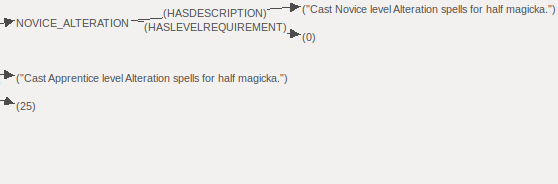
\includegraphics[scale=1]{abox_adept_alteration_p2}
\end{figure}

In the images above we can see the ADEPT\_ALTERATION skill and its traits: the hasLevelRequirement attribute being 50, the perk description being "Cast Adept level Alteration spells for half magicka." and its skill requirement being the APPRENTICE\_ALTERATION. After that we can see how it unrolls until it reaches NOVICE\_ALTERATION, which has no skill requirement left.


\clearpage
\section{Rules}
In our ontology we defined one rule to sort skills into the \textit{NOT\_UPGRADEABLE} category. This was necessary since our skills can only belong to one of the two categories: \textit{UPGRADEABLE} or \textit{NOT\_UPGRADEABLE}. Using this rule made it easier for us to build the ontology since out of the 180 skills only 27 are upgradeable. After defining the rule, we run it to activate it.

\begin{lstlisting}
(define-rule (?x NOT_UPGRADEABLE) (and (?x SKILL) (neg (?x UPGRADEABLE))))

(run-all-rules)
\end{lstlisting}

%\clearpage
\section{Queries}
The last thing we do as part of loading the ontology and before we run our queries is running all the rules with the \textit{run-all-rules} command. After this step, we can run our evaluation queries.
We check the consistency of our ontology with the following queries.

\begin{lstlisting}
(abox-consistent?)
(tbox-cyclic?)
(tbox-coherent?)

(realize-abox)
(classify-tbox)
\end{lstlisting}

Then we check the size of our ontology with the following queries.

\begin{lstlisting}
(evaluate (length (all-individuals)))
(evaluate (length (all-atomic-concepts)))
(evaluate (length (all-roles)))
(evaluate (length (all-rules)))

(all-concept-assertions)
(all-role-assertions)
(all-constraints)

(describe-tbox)
(describe-abox)

(taxonomy)
\end{lstlisting}

Then we check the expressivity of our ontology with the following queries.

\begin{lstlisting}
(get-tbox-language)
(get-abox-language)

(all-features)
(all-transitive-roles)
\end{lstlisting}

Finally we answer some of the competency question we extracted previously with the following queries.

\begin{itemize}
\item What are the races of characters I can play?
\begin{lstlisting}
(concept-instances RACE)
\end{lstlisting}

\item What are the skills suitable for build X?
\begin{lstlisting}
(individual-fillers PRIEST (inv isSuitable))
\end{lstlisting}

\item Should I invest in skill class X if my character is build Y?
\begin{lstlisting}
(individuals-related? ONE_HANDED PRIEST isSuitable)
\end{lstlisting}

\item What skills can I unlock at level X?
\begin{lstlisting}
(retrieve (?x) (and (?x SKILL) (?x (equal hasLevelRequirement 50))))
\end{lstlisting}

\item What skill is required for unlocking skill X?
\begin{lstlisting}
(individual-fillers POWER_BASH hasSkillRequirement)
\end{lstlisting}

\item What level is required for unlocking skill X?
\begin{lstlisting}
(individual-told-attribute-value BACKSTAB hasLevelRequirement)
\end{lstlisting}

\item What are the perks provided by skill X?
\begin{lstlisting}
(individual-told-attribute-value DISINTEGRATE hasDescription)
\end{lstlisting}
\end{itemize}


\clearpage
\appendix

\chapter{Original code}
\section{Racer ontology}
\lstinputlisting{../onto.racer}


\section{Racer evaluation}
\lstinputlisting{../evaluation.racer}


%\printbibliography

\vspace{2cm}
\begin{center}
Intelligent Systems Group\\
\pgfimage[width=10cm]{fig/footer}
\end{center}



\end{document}
